\newpage
\section{Fluid discretization}
\label{sec:fluid-discretization}

This Section presents an attempt at discretizing Equations \eqref{eq:navier_cont} and \eqref{eq:navier_momentum}. With most particulate Lagrangian methods that is to say that the equations will be written with the corresponding discrete operators, in our case, the ones introduced in Section \ref{Subsec:discrete_interp}.

The continuity equation \eqref{eq:navier_cont} is traditionally discretized by employing the notion that $\rho \ve{\nabla} \cdot \ve{u} = \ve{\nabla} \cdot( \rho \ve{u}) - \ve{u} \cdot\ve{\nabla} \rho$, rendering equation \eqref{eq:navier_cont} as 
%
\begin{equation} \label{eq:sph_navier_cont}
	\frac{{d\rho_i }}{{dt}} = \sum_j{{m_j} \ve{u}_{ij} \cdot \ve{\nabla} W(\ve{r}_{ij}, h)}
\end{equation}
%
This is the equivalent of applying operator \eqref{eq:discr_interp_4} to approximate the $\ve{\nabla} \cdot \ve{u} $ field and taking $\Phi=\rho$. Equation \eqref{eq:sph_navier_cont} produces a zero divergence field for a constant $\ve{u}$ field. 

The approach of Sections \ref{Subsec:Interpolation} and \ref{Subsec:discrete_interp} was consistent with the designing of interpolation operators that would provide a desired accuracy. In particle methods, however, it becomes trivial and very tempting to interpret any equation in terms of pair-wise interaction between particles. For that purpose, we can agree that 

%
\begin{equation} \label{eq:physical_interp_I}
	\ve{\nabla} W(\ve{r}_{ij}, h) = \ve{r}_{ij}F(\ve{r}_{ij}, h)
\end{equation}
%
where $F(\ve{r}_{ij}, h) \leq 0$ is a function that respects Equation \eqref{eq:physical_interp_I}. The contribution of particle $j$ to the density variation of particle $i$ is then

%
\begin{equation} \label{eq:physical_interp_II}
	m_j\ve{u}_{ij} \cdot \ve{r}_{ij}F(\ve{r}_{ij}, h)
\end{equation}
%
This implies that approaching $ij$ particles i.e., for $\ve{u}_{ij} \cdot \ve{r}_{ij} \leq 0$, the interaction contributes with a positive density change, as our physical intuition expects. Equation \eqref{eq:sph_navier_cont} describes a medium that allows density changes, i.e., it is compressible. By allowing for \textit{some} compressibility the presented discretization is usually called \ac{WCSPH}. It has become the traditional \ac{SPH} way of modeling incompressible flows \citep{Monaghan-2005, Lee-2010}. Implementation is trivial since pressure is obtained from a \ac{EOS}, written so that the speed of sound is large enough to keep the relative density fluctuations small. \cite{Lee-2010} gives good insight into the relative accuracy of the pressure field of both \ac{WCSPH} and an incompressible approach, with the later being superior in most situations. Forcing incompressibility however, demands the solution of a large and potentially sparse Poisson problem at every time-step, built by defining a boundary at the free surface, that needs to be traced accurately. When dealing with highly distorted flows this is a major computational drawback and undermines the Lagrangian nature of the calculation. More details of the \ac{WCSPH} formulation are discussed in Section \ref{sec:eos}.

The pressure gradient of the Navier-Stokes equation (\eqref{eq:navier_momentum}) can be discretized in a number of ways. \cite{Gingold-1982} and \cite{Violeau-2012} used the discrete approximation of the Lagrangian of a particle system, using operators \eqref{eq:discr_interp_2} and \eqref{eq:discr_interp_4}. The same operators can be used directly to discretize the term in Equation \eqref{eq:navier_momentum}, leading to

%
 \begin{equation} \label{eq:sph_pressure_momentum}
\frac{\ve{\nabla}p_i}{\rho_i} = \sum_j{m_j \left( \frac{p_i}{\rho_i^2} +\frac{p_j}{\rho_j^2}\right) \ve{\nabla} W(\ve{r}_{ij}, h)},
\end{equation}
%
\noindent a symmetrical, balanced form of the pressure term that respects the action reaction principle. This implies that linear and angular momentum are conserved exactly by \eqref{eq:sph_pressure_momentum}. The second term of the second member in Equation \eqref{eq:navier_momentum} refers to the shear stresses, and it involves a second derivative of the velocity. As mentioned in Section \ref{Subsec:discrete_interp}, applying the SPH operators directly to the second derivative is avoided since it is too sensitive to particle disorder and limits the choice of the kernel functions. 

Three approaches to modeling this term are presented: the artificial viscosity model introduced by \cite{Gingold-1982}, the laminar viscosity model by introduced by \cite{Morris-1997} and the \ac{SPS} terms, properly presented in \cite{Dalrymple-2006} and discussed in Section \ref{sec:sps}.

\cite{Gingold-1982} introduced a momentum dissipating term in the form of a viscosity, designed to treat shock-tube problems. This form of numerical viscosity also mitigates problems due to instabilities arising in the system coming from the unstructured behavior of the particles, as well as accumulation of acoustic energy from integration errors during a simulation without dissipation. It is written as
%
\begin{equation}
\begin{split} 
\label{eq:sph_artificial_visc_I}
{
\ve{\Pi} _{i}} = \sum_j\left\{ {\begin{array}{*{20}{c}}
  {\frac{ \displaystyle { - \alpha {{\bar c}_{ij}}{\mu _{ij}}}}{\displaystyle {{{\bar \rho }_{ij}}}}\ve{\nabla}W(\ve{r}_{ij}, h)} \\ \\
  0 
\end{array}} \right.{\text{    }}\begin{array}{*{20}{c}}
  \text{if}\;\;\;{{{\ve{u}}_{ij}}\cdot{{\ve{r}}_{ij}} < 0} \\ \\
  \text{if}\;\;\;{{{\ve{u}}_{ij}}\cdot{{\ve{r}}_{ij}} \geqslant 0} 
\end{array} \;\;\; 
\hbox{with} \;\;\; {\mu _{ij}} = \frac{{({{\ve{u}}_{ij}}\cdot{{\ve{r}}_{ij}}}h)}{{{{r}}_{ij}^2}},
\end{split}
\end{equation}
%
\noindent where $c$ is the sound celerity and $\alpha$ is a parameter subject to calibration. This expression is traditionally used due to its simple implementation, conservation of linear and angular momentum and because it converges to $\mu {\ve{\nabla}^2}{\ve{u}}$ as $h \rightarrow 0$ \citep{Issa-2004}. It is however considered dissipative regarding shear and vorticity, and the case-dependent $\alpha$ parameter confirms its empirical nature.

\cite{Morris-1997}, influenced by the work of \cite{Cleary-1996}, proposed to model the shear viscosity by 

\begin{equation} \label{eq:sph_morris_laminar}
	\ve{\Pi}_{i} = \sum_j m_j \left( \frac{4\nu \ve{r_}{ij} \cdot \ve{\nabla}W(\ve{r}_{ij}, h) }{(\rho_i + \rho_j){{r}}_{ij}^2} \right)\ve{u}_{ij} 
\end{equation}
%
where $\nu$ is the actual kinematic viscosity of the fluid, defined as $\nu=\mu/\rho$. This expression conserves linear momentum but not angular momentum \citep{Colagrossi-2011}. Recent ideas over the local consistency of Expression \eqref{eq:sph_morris_laminar}, particularly in when the kernel is truncated, have been discussed by \cite{Colagrossi-2011} and \cite{Gonzalez-2009}.


The momentum equation (\eqref{eq:navier_momentum}) can now be written as
%\begin{equation} \label{eq:sph_navier_momentum}
%\begin{split}
%	\frac{{d{\boldsymbol{v}_i}}}{{dt}} = -\sum_j{m_j \left( \frac{p_i}{\rho_i^2} +\frac{p_j}{\rho_j^2} \right) \boldsymbol{\nabla} W(\boldsymbol{r}_{ij}, h)} +\\+ \sum_j m_j \left( \frac{4\mu \boldsymbol{r_{ij}} \boldsymbol{\nabla}W(\boldsymbol{r}_{ij}, h) }{(\rho_i + \rho_j)(|r_{ij}|^2 +\eta^2 )} \right)\boldsymbol{v}_{ij} + \sum_j{m_j \left( \frac{\tau_i}{\rho_i^2} +\frac{\tau_j}{\rho_j^2} \right) \boldsymbol{\nabla} W(\boldsymbol{r}_{ij}, h)} + {{\boldsymbol{g}}} 
%\end{split}
%\end{equation}
%%
\begin{equation} \label{eq:sph_navier_momentum_I}
	\frac{{d{\boldsymbol{u}_i}}}{{dt}} = -\sum_j{m_j \left( \frac{p_i}{\rho_i^2} +\frac{p_j}{\rho_j^2} \right) \boldsymbol{\nabla} W(\boldsymbol{r}_{ij}, h)} + \ve{\Pi}_{i} + \ve{g}
\end{equation}
%


%%%%%%%%%%%%%%%%%%%%%%%%%%%%%%%%%%%%%%%%%%%%%%%%%%%%%%%%%%%%
\subsection{Turbulence modeling}
\label{sec:sps}

Expressions \eqref{eq:sph_artificial_visc_I} and \eqref{eq:sph_morris_laminar} attempt to account for shear stresses developed at the scale of the interparticle interactions, $h$. Turbulent fluid flow however, may present very small local scales, depending on the Reynolds number, $R_e$ \citep{Batchelor-2000, pope-2000}. Attempting to model all of these scales is designated by \ac{DNS}, where no turbulent closures are needed. This imposes a serious limit on the range of possible $R_e$, since computational resources are limited. Opposite to this, the \ac{RANS} rely on closure models to estimate the stresses that arise even from large, energy-carrying structures. Another approach naturally compatible with our framework is to use \ac{LES} techniques, that can be understood as a intermediate between \ac{DNS} and \ac{RANS}. The idea is that the governing equations are spatially averaged over a length scale of the order of the numerical discretization. The contribution of the large structures to momentum and energy transfer is computed directly and only the effects of the smallest scales of turbulence are modeled. The hope is that, since the small scales tend to be more homogeneous and universal \citep{pope-2000}, the models can be simpler and require fewer adjustments when applied to different flows than similar models for the \ac{RANS}. 

To obtain the motion equations of the resolved scales, large and small scales must be separated. \ac{LES} is based on the definition of a filtering operation: a resolved variable is defined as

%
\begin{equation} \label{eq:eq_les_filter}
	\left\langle A \right\rangle(\ve{r})=\int_\Omega{A(\ve{r}')G\left( {{\ve{r}}, {\ve{r}}';\left\langle \Delta \right\rangle} \right)d{\ve{r}}'}  , 
\end{equation}
%
where $G$ is the filter function, the $\left\langle \; \right\rangle$ operator represents a generic spatial averaging and $\left\langle \Delta \right\rangle$ is the filter-width associated with the wavelength of the smallest scale retained by the filtering operation. Thus, the filter function determines the size and structure of the small scales. A special note should be given regarding the idea of the integral interpolant behind \ac{SPH} (Equation \eqref{eq:interpolant_1}) and the filtering operation of \ac{LES}. Since both \ac{SPH} and \ac{LES} share the same mathematical structure, it should come as no surprise that the combination of the methods seems very atractive to modelers.

\cite{Gotoh-2001} introduced this type of subgrid scaling for their incompressible \ac{MPS} method, as did \cite{Lo-2002} for their incompressible SPH method. For a compressible fluid, sub-particle scaling requires the use of special averaging, with Favre-averaging being the typically chosen in the literature. It is written as

%
\begin{equation} \label{eq:favre-average}
	\left\langle A \right\rangle=\frac{\left\langle\rho A\right\rangle}{\left\langle\rho\right\rangle}
\end{equation}
%
By using Favre-averaging, no new terms are introduced in the conservation equations, except for the \ac{SPS} terms. This means that Equations \eqref{eq:sph_navier_cont} and \eqref{eq:sph_navier_momentum_I} are implicitly in their filtered form, assuming $\left\langle A \right\rangle=A$\footnote{An acceptable abuse of notation since the averaged scale is indeed our working scale, no ambiguity is introduced.}. For the momentum Navier-Stokes equation, the application of a flat-top spatial filter yields \citep{Yoshizawa-1986} 

%
\begin{equation} \label{eq:navier_momentum_filtered}
		\frac{d\left\langle\ve{u}\right\rangle}{dt}= -\frac{1}{\left\langle\rho\right\rangle}\ve{\nabla}\left\langle p\right\rangle + \frac{1}{\left\langle\rho\right\rangle}\mu \ve{\nabla}^2\left\langle\ve{u}\right\rangle + \frac{1}{\left\langle\rho\right\rangle} \ve{\nabla}\cdot\ve{\tau}^* + \ve{g},
\end{equation}
%
where $\ve{\tau}^*$ is the \ac{SPS} tensor. Several proposals exist for the form of the tensor. Eddy-viscosity models try to reproduce the global exchange of energy between the resolved and unresolved stresses by mimicking the drain of energy associated with the turbulence energy cascade \citep{Batchelor-2000}. \cite{Yoshizawa-1986} proposed an eddy-viscosity model for weakly compressible turbulent flows using a multiscale direct-interaction approximation method. The anisotropic part of the \ac{SPS} is parametrized using the Smagorinsky (1963) model, while the \ac{SPS} energy is modeled by a  separate term

%
\begin{equation} \label{eq:sph_sps_visc}
	\frac{\ve{\tau}^*}{\left\langle\rho\right\rangle} = 2\nu_t \left( \left\langle\ve{D}\right\rangle - \frac{1}{3}\ve{\delta}\text{tr}\left(\left\langle\ve{D}\right\rangle\right) \right) - \frac{2}{3}C_I \Delta^2\ve{\delta}|\left\langle\ve{D}\right\rangle|^2,
\end{equation}
%
where $\nu_t=(C_S\Delta)^2|\left\langle\ve{D}\right\rangle|$ is the eddy viscosity, $C_S=0.1677$ is the Smagorinsky constant, $C_I=6.6\times10^{-3}$ and  $|\left\langle\ve{D}\right\rangle|=(2\left\langle\ve{D}\right\rangle\left\langle\ve{D}\right\rangle)^{1/2}$ \citep{Martin-al-2000}.

 
In \ac{SPH} notation, the \ac{SPS} term receives the same treatment as the pressure gradient term, in Equation \eqref{eq:sph_pressure_momentum}:

%
 \begin{equation} \label{eq:sph_sps_term}
\ve{\Pi}^{SPS}_{i} = \sum_j{m_j \left( \frac{\ve{\tau}^*_i}{\rho_i^2} +\frac{\ve{\tau}^*_j}{\rho_j^2}\right) \cdot \ve{\nabla} W(\ve{r}_{ij}, h)},
\end{equation}
%
where strain rate tensor is computed directly by approximating the velocity gradients with operator \eqref{eq:discr_interp_4} ($\Phi=\rho$). The $\Delta$ filter-width is typically taken as the distance between particles.


%%%%%%%%%%%%%%%%%%%%%%%%%%%%%%%%%%%%%%%%%%%%%%%%%%%%%%%%
\subsection{Density and pressure fields}
\label{sec:eos}

The \ac{WCSPH} formulation introduced by Equation \eqref{eq:sph_navier_cont} demands the usage of an \ac{EOS} to link the pressure and density fields. The most commonly employed \ac{EOS} is called Tait's Equation \citep{Batchelor-2000}, and is usually used to describe barotropic fluids:

%
\begin{equation} \label{eq:sph_state_equation}
	p_i = \frac{\rho_0 C_s^2}{\gamma} \left[ \left( \frac{\rho_i}{\rho_0} \right)^{\gamma} -1 \right]
\end{equation}
%
\noindent where $\rho_0$ is a reference density, $C_s$ is the numerical sound celerity and $\gamma=7$ for a fluid like water. It is used for free-surface flow because it assumes negligible atmospheric, or background, pressure.
$C_s=\sqrt{\partial p / \partial \rho}|_{\rho_0}$ \citep{Batchelor-2000} can be chosen large enough to render relative density fluctuations small, i.e., since

%
\begin{equation} \label{eq:sph_state_equation_cs}
	\frac{|\delta\rho_i|}{\rho_i} \sim \frac{u_i^2}{C_s^2}
\end{equation}
%
$C_s$ can be chosen as any percentage of the maximum velocity in the flow to ensure that the maximum density fluctuation is one order of magnitude lower. Typically $C_s$ is taken as $10\max u_i$, guaranteeing that $\max({|\delta\rho_i|}/{\rho_i}) \sim 0.01$. By using the first term of a Taylor expansion of Equation \eqref{eq:sph_state_equation_cs}, a linearized \ac{EOS} can be written as

%
\begin{equation} \label{eq:sph_state_equation_linear}
	p_i = {C_s^2}(\rho_i-\rho_0)
\end{equation}
%
This is built assuming locally smooth density gradients, and is usually used in the absence of a free-surface.

Equation \eqref{eq:sph_state_equation} represents a very stiff density field, and together with the natural disordering of the Lagrangian particles, high-frequency low amplitude oscillations are found to populate the density scalar field \citep{Molteni-2009}. The explored strategy in this work is to use a diffusive term in the continuity equation, now written as

%
\begin{equation} \label{eq:sph_navier_cont_delta_sph}
	\frac{{d\rho_i }}{{dt}} = \sum_j{{m_j} \ve{u}_{ij} \cdot \ve{\nabla} W(\ve{r}_{ij}, h)+\Phi_i}
\end{equation}
%
where

%
\begin{equation} \label{eq:delta_sph_molteni}
	\Phi_i =  2 \delta_\Phi h C_s \sum_j{(\rho_j-\rho_i) \frac{\ve{r}_{ij} \cdot \ve{\nabla} W(\ve{r}_{ij}, h)}{{r}_{ij}^2} \frac{m_j}{\rho_j}},
\end{equation}
%
This represents the original $\delta$-\ac{SPH} formulation by \cite{Molteni-2009}, due to the free parameter $\delta_\Phi$, that needs to be attributed a suitable value. It can be explained simply as the addition of the Laplacian of the density field to the continuity equation. \cite{Antuono-2012} has presented a careful analysis of the influence of this term in the system, by decomposing the Laplacian operator, observing the converge of the operators and performing linear stability analysis to inspect the influence of the $\delta_\Phi$ diffusive coefficient. Equation \eqref{eq:delta_sph_molteni} represents exactly a diffusive term in the domain bulk. The behavior changes close to open boundaries such as free-surface. Due to truncation of the kernel (there are no particles being sampled outside of an open boundary), the first order contributions of \eqref{eq:delta_sph_molteni} are not null \citep{Antuono-2010}, resulting in a net force applied to the particles. This effect is not considered relevant for non-hydrostatic situations, where this force is many orders of magnitude inferior to any other force involved. Corrections to this effect were proposed by \cite{Antuono-2010}, but involve the solution of a renormalization problem for the density gradient, with considerable computational cost.



%%%%%%%%%%%%%%%%%%%%%%%%%%%%%%%%%%%%%%%%%%%%%%%%%%%%%%%%
\subsection{Boundary Conditions}
\label{sec:BCs}

Boundary conditions must respect the ideas developed in Section \ref{subsec:boundary_cond}, particularly, that continuity of stresses across any interface must be respected. Another apparent advantage of particulate methods is that the condition is inherently satisfied since particles will respect Equations \eqref{eq:navier_cont} and \eqref{eq:navier_momentum} via their discrete forms, Equations \eqref{eq:sph_navier_cont} and \eqref{eq:sph_navier_momentum_I}. In \ac{SPH} however, the kernel is truncated near the boundaries and the imposition of a correct stress field at solid interfaces is demanding. The typical attempt at a solution is to complete the kernel on these regions, by introducing a series of boundary particles that may respect a different set of equations. Four major approaches are used for this effect: i)ghost particles, ii)repulsive particles, iii)dynamic particles and iv)boundary integrals. 

Ghost particles were initially devised by \cite{Randles-1996} in order to respect a no-slip condition at the same time that the kernel is not truncated. If a fluid particle is close to a solid boundary, for ($r_{ij}<h$), a new particle is generated as the specular image of the incident one, as the scheme in Figure \ref{fig:Ghost_particles}. 
%
\begin{figure}[H]
	\centering
	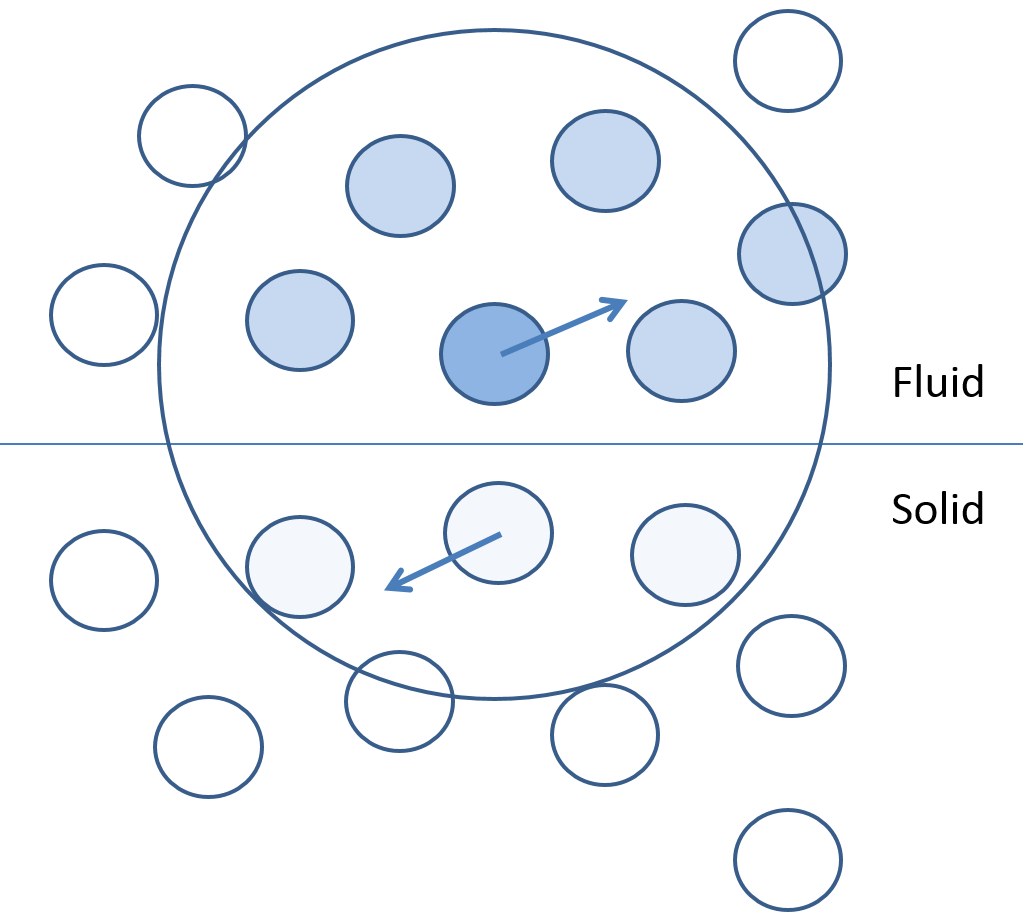
\includegraphics[width=0.45\linewidth]{Figures/3.Chapter/Ghost_particles}
	\caption{Scheme of ghost particles boundary condition.}
	\label{fig:Ghost_particles} 
\end{figure}
%

Both particles have the same density, but opposite normal and tangential velocities. Two disadvantages arise with this approach: complex geometries are extremely difficult to model (sharp angles, thin plates, hollow boxes) and the number of particles in the system may vary at each time step, a further implementation complication, explored in Section \ref{cap:chapter_hpc}. 


Repulsive particles \citep{Monaghan-1999} represent stationary particles that do not respect the conservation equations, but instead apply \textit{ad-hoc} forces to approaching fluid particles. The forces may be based on Lennard-Jones potentials, and a series of interpolation procedures are carried out to assure the continuity of a force field perceived by a fluid particle moving in an arbitrary direction from the boundary, as represented in Figure \ref{fig:repulsive_particles}.
%
\begin{figure}[H]
	\centering
	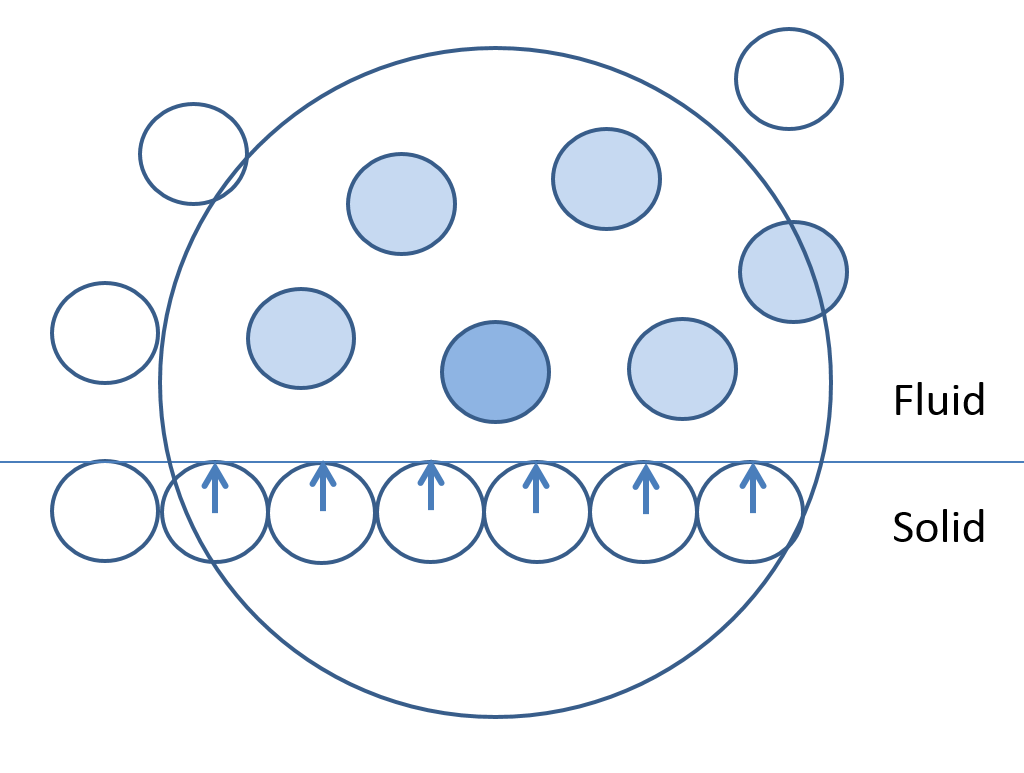
\includegraphics[width=0.45\linewidth]{Figures/3.Chapter/Repulsive_particles}
	\caption{Scheme of repulsive particles boundary condition.}
	\label{fig:repulsive_particles} 
\end{figure}
%

Dynamic particles were introduced by \cite{Dalrymple-2000} and further studied by \cite{Crespo-2007}, that devised them as fluid particles with an externally imposed motion. The particles respect Equations \eqref{eq:sph_navier_cont} and \eqref{eq:sph_navier_momentum_I} but their position is not given by integrating the velocity in time. A static boundary will have zero velocity (traditional arrangement in Figure \ref{fig:Dynamic_particles}) and a moving boundary will have a prescribed motion.
%
\begin{figure}[H]
	\centering
	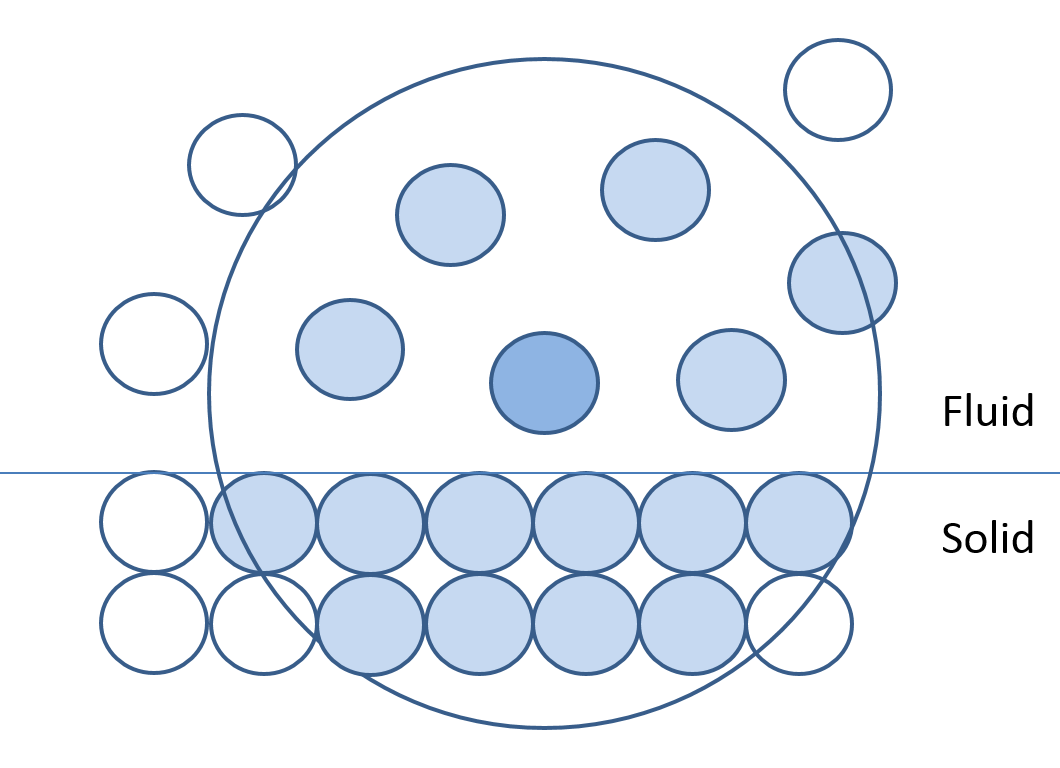
\includegraphics[width=0.45\linewidth]{Figures/3.Chapter/Dynamic_particles}
	\caption{Scheme of dynamic particles boundary condition.}
	\label{fig:Dynamic_particles} 
\end{figure}
%

A known difficulty of this formulation is the overestimation of the density \citep{Price-2008,Saitoh-2013}, resulting from an entropy jump across the fluid/solid interface. This results in an increased distance of fluid-solid particles due to the added force from the pressure gradient, effectively disturbing the viscous forces computed at that interface \citep{Colagrossi-2003}.

Boundary integral ideas are being explored in order to complete the kernel around boundaries, namely, analytically summing the missing terms. The boundary integral conditions \citep{Ferrand-al-2013, Mayrhofer-al-2015} are promising but still face many challenges related to complex geometries and efficient implementations.

This work will employ dynamic boundary conditions throughout, due to the simplicity and potential of the implementation. The solid body discretization presented in Section \ref{sec:solid-discretization} will also use the same framework.



